% This is LLNCS.DEM the demonstration file of
% the LaTeX macro package from Springer-Verlag
% for Lecture Notes in Computer Science,
% version 2.4 for LaTeX2e as of 16. April 2010
%
\documentclass{llncs}
%
\usepackage{makeidx}  % allows for indexgeneration
\usepackage[LY1]{fontenc}
\usepackage[utf8]{inputenc}
\usepackage{ctable}
\usepackage{multirow}
\usepackage{hhline}
\usepackage{cite}
%\usepackage{algorithmicx}
\usepackage{algorithmic}
\usepackage{algorithm}
%\usepackage{algpseudocode}
\usepackage{xcolor}

%
\begin{document}
%
\frontmatter          % for the preliminaries
%
\pagestyle{headings}  % switches on printing of running heads
\addtocmark{Hamiltonian Mechanics} % additional mark in the TOC
\newcommand{\junk}[1]{}

%
%\tableofcontents
%
\mainmatter              % start of the contributions
%
\title{Improving genome assemblies using multi-platform sequence data}
%
\titlerunning{Improving genome assemblies}  % abbreviated title (for running head)
%                                     also used for the TOC unless
%                                     \toctitle is used
%
\author{Pınar Kavak\inst{1,2,*} \and Bekir Ergüner\inst{1}
Duran Üstek\inst{3} \and Bayram Yüksel\inst{4} \and Mahmut Şamil Sağıroğlu\inst{1} \and Tunga Güngör\inst{2} \and Can Alkan\inst{5,*}}
%

\authorrunning{Pınar Kavak et al.} % abbreviated author list (for running head)
%
%%%% list of authors for the TOC (use if author list has to be modified)
\tocauthor{Pınar Kavak, Bekir Ergüner, Duran Üstek, Bayram Yüksel, Mahmut Şamil Sağıroğlu, Tunga Güngör, Can Alkan}
%
\institute{Advanced Genomics and Bioinformatics Research Group (İGBAM), BİLGEM, The Scientific and Technological Research Council of Turkey (TÜBİTAK),\\
41470 Gebze, Kocaeli, Turkey\\
\email{pinar.kavak@tubitak.gov.tr}
\and
Department of Computer Engineering,
Boğaziçi University,\\ 
34342 Bebek, İstanbul, Turkey
\and
Department of Medical Genetics, 
İstanbul Medipol University,\\
34810 Beykoz, İstanbul, Turkey
\and
TÜBİTAK - MAM - GMBE (The Scientific and Technological Research Council of Turkey, Genetic Engineering and Biotechnology Institute),\\
41470 Gebze, Kocaeli, Turkey
\and
Department of Computer Engineering, 
Bilkent University,\\
06800 Bilkent, Ankara, Turkey\\
\email{calkan.cs.bilkent.edu.tr}
}


\maketitle              % typeset the title of the contribution

\begin{abstract}
Accurate \textit{De novo} assembly using short reads generated by next generation sequencing technologies is still an open problem. Although there are several assembly algorithms developed for data generated with different sequencing technologies, and some that can make use of hybrid data, the assemblies are still far from being perfect. There is still a need for computational approaches to improve draft assemblies.
Here we propose a new method to correct assembly mistakes when there are multiple types of data generated using different sequencing technologies that have different strengths and biases. We exploit the assembly of highly accurate short reads to correct the contigs obtained from less accurate  long reads.
We apply our method to Illumina, 454, and Ion Torrent data, and also compare our results with existing hybrid assemblers, Celera and Masurca.
\keywords{\textit{de novo} assembly, assembly improvement, next generation multi-platform sequencing}
\end{abstract}
%
\section{Scientific Background}
Since the introduction of high throughput sequencing (HTS) technologies, traditional Sanger sequencing is being abandoned especially for large-scale sequencing projects.
Although cost effective for data production, HTS also imposes increased cost for data processing and computational burden. 
In addition, the data quality is in fact lower, with greater error rates, and short read lengths for most platforms. 
One of the main algorithmic problems to analyze HTS data is the \textit{de novo} assembly: i.e. ``stitching'' billions of short DNA strings into a collection of larger sequences, ideally the size of chromosomes. 
However, ``perfect'' assemblies with no gaps and no errors are still lacking due to many factors, including the short read and fragment (paired-end) lengths, sequencing errors in basepair level, and the complex and repetitive nature of most genomes. 
Some of these problems in \textit{de novo} assembly can be ameliorated through using data generated by different sequencing platforms, where each technology has ``strengths'' that may be used to fix biases introduced by others.

There are three kinds of assemblers mainly used to do genome assembly: i) greedy assemblers \cite{ssake:2007,sharcgs:2007,vcake:2007}, ii) overlap-layout-consensus (OLC) graph based assemblers \cite{celera:2000, sga:2012, hapsemblerDonmez:2011} and de Bruijn graph based assemblers \cite{eulerPevzner:2008, abyssSimpson:2009, velvetZerbino:2008, spadesBankevich:2012, allpaths:2008}. Greedy assemblers follow a greedy approach  as follows: given one read or contig,  at each step assembler adds one more read or contig with the largest overlap. The problem of greedy assemblers is that they can get stuck at local maxima. Therefore they are generally used for small genome assemblies. Since they also use more memory and are slower, it is not feasible to assemble large genomes with greedy assemblers.
OLC graph based assemblers work well when the long reads are available for assembly. They generate all-against-all pairwise alignments and build the graph by representing reads as nodes and overlaps between reads as edges. 
They obtain the consensus assembly by following a Hamiltonian path on the graph. 
Assemblers that are based on de Bruijn graphs are designed primarily for short reads. 
They use a k-mer graph approach rather than calculating all-against-all pairwise alignments. They build the graph by using k-mers as edges and the overlaps between k-mers as nodes. They follow an Eulerian path through the k-mer graph to find a consensus assembly.
Several assemblers use multiple read libraries \cite{cabogMiller:2008, masurcaZimin:2013, miraest, cerulian:2013} for better assembly construction. CABOG \cite{cabogMiller:2008} is at first designed for Sanger sequencing, it is then revised to use 454 data, but it also accepts Illumina data to 
generate a hybrid assembly. Masurca \cite{masurcaZimin:2013} is able to assemble Illumina reads   together with longer 454 and Sanger reads. MIRAest \cite{miraest} can use Sanger, 454, Illumina, Ion-Torrent and corrected PacBio data for hybrid assembly. It works on small genomes. Cerulean \cite{cerulian:2013} uses long PacBio reads and short Illumina reads to construct a hybrid assembly. It uses \textit{assembly graphs} generated by ABySS \cite{abyssSimpson:2009} assembler with paired end Illumina reads and the mapping of long PacBio reads to the assembled contigs, as inputs.

Additionally, strategies to merge different assemblies using different data sources into a single coherent assembly are described in the literature (e.g. \cite{wang:2012}). Our method differs from that of \cite{wang:2012}, in data types. \cite{wang:2012} works on Illumina, 454 and ABI SOLID data, where we work on Illumina, 454 and Ion-Torrent data. Also pre- and post-processing steps of the two methods differ. \cite{wang:2012} at first assembles 454, Illumina and SOLID data separately with different assemblers and then assembles the resulting contig collection again with another assembler.

In this work, we propose a method to improve draft assemblies (i.e. produced using a single data source, and/or single algorithm) by incorporating data generated by different HTS technologies, and applying novel correction methods. To achieve better improvements, we exploit the advantages of both short but low-error-rate reads and long but erroneous reads. 
We show that correcting the contigs built by assembling long reads through mapping short and high quality read contigs produce the best results, compared to the assemblies generated by algorithms that use hybrid data all at once. With this study, we also have the opportunity to compare Ion-Torrent and Roche/454 reads in terms of assembly performances.

\section{Materials and Methods}
\label{meth}
A part of human chromosome 13 was cloned into a bacterial artificial chromosome (BAC) in a previous study. 
We sequenced the BAC clone separately using Illumina, Roche/454, and Ion-Torrent platforms. Data properties are given in Table \ref{tab:dataprop}. A ``gold standard'' reference assembly was also obtained using template-based assembly with Mira~\cite{mira} using Roche/454 data, which is then corrected using the Illumina reads\cite{BACRef}. Since Roche/454 and Ion Torrent platforms have similar sequencing biases (i.e. problematic homopolymers), we separated this study into two different groups: Illumina \& 454 and Illumina \& Ion-Torrent. We applied the same method on the two groups and evaluated them separately which gave us the opportunity to compare Roche/454 and Ion-Torrent data. The flowchart of the pipeline is shown on Figure \ref{flowChart}.

\ctable[
      cap     = {},
      % 
      caption = {Properties of the data},
      % 
      label   = {tab:dataprop},
      doinside = \normalsize,
      width = 0.95\textwidth,
      %
      %
      pos = h!tb,
      star
]      {>{\raggedright\arraybackslash}X>{\raggedright\arraybackslash}X>{\raggedright\arraybackslash}
X>{\raggedright\arraybackslash}X>{\raggedright\arraybackslash}}
{
      \tnote[]{{\scriptsize \textbf{Technology}: The name of the sequencing technology used to produce the reads.
      \textbf{Length range}: Minimum and maximum lengths of the generated reads.
      \textbf{Mean length}: The mean length among all reads.
      \textbf{Mean base qual}: The average phred score sequence quality of all reads. Calculated by summing up all phred scores of the bases in a read and dividing it to sequence length of the read, over all reads.
      \textbf{Paired:} Represents whether the sequencing is performed as paired-end or single-end.}}
}
{ \FL
Technology & Length range & Mean length & Mean base qual (phred s.) & Paired \\ \ML
Illumina & 101bp \footnotesize{(all reads have equal length)} & 101bp & 38 & paired \\
\addlinespace[1mm]
Roche/454 & 40bp-1027bp & 650bp & 28 & single-end \\
\addlinespace[1mm]
Ion-Torrent & 5bp-201bp & 127bp & 24 & single-end \\
\LL
}

\subsection{Pre-processing} 
Pre-processing steps consist of the following: 
\begin{itemize}
\item First, the reads that have low average quality value (phred score 17, i.e. $\geq$2\% error rate) were discarded. 
\item Then, the reads with high N-density (with $>$10\% of the read consisting of Ns) were removed. 
\item Third, groups of bases that seem to be non-uniform according to sequence base content (A,T,G,C) were trimmed (See Figure \ref{nonuniformATGC}). 
\item Finally, each assembler's pre-processing operations were also inevitably applied.
\end{itemize}

\begin{figure*}[htbp]
\centerline{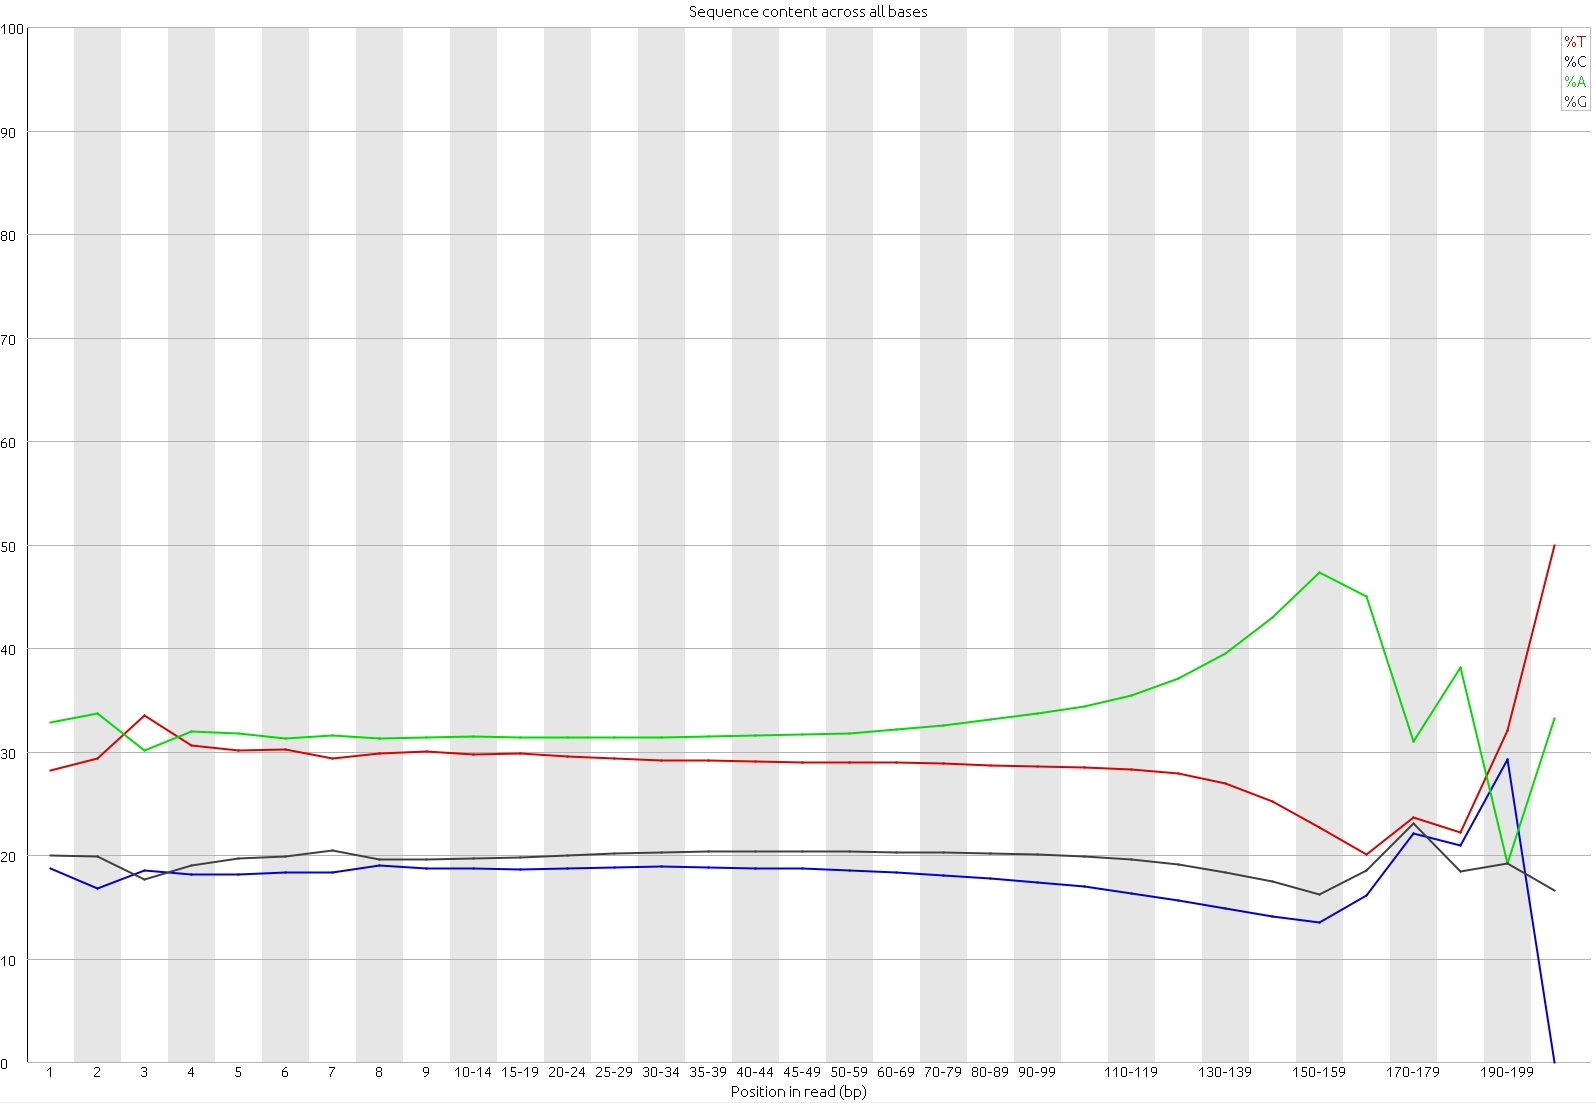
\includegraphics[width=12cm, height=5cm]{ionTorrentFastqc.jpg}}
\caption{Non-uniform A,T,G,C regions of Ion-torrent reads. First 8 bases and the bases after 130th base are trimmed in pre-processing.}
\label{nonuniformATGC}
\end{figure*}

\subsection{Assembly} 
After the pre-processing, we used several proper assembly tools to assemble different types of data: Velvet~\cite{velvetZerbino:2008}, a de Bruijn graph based assembler that is designed to assemble the short reads, is used for the assembly of Illumina reads. Considering the trimmed beginning and/or end parts of 101bp long paired-end reads from Illumina, and after testing kmers 21 and 31, we decided to use kmer=51 for the short read assembly. We ran Velvet with shortPaired mode with insert size 400bp, expected coverage 80, coverage cutoff 2, minimum contig length 100. N50 value of the resulting short read contigs was 8,865. We used two different OLC assemblers: Celera~\cite{celera:2000}, and SGA~\cite{sga:2012} to assemble the long read data sets (Roche/454 and Ion Torrent) separately. We ran Celera assembler with unmated mode and with default parameters to assemble 454 and Ion-Torrent reads. N50 value of the assembly obtained with 454 and Ion-Torrent reads with Celera was 1,308 and 1,284 respectively. We also used SGA assembler with unmated mode for the same purpose. We obtained N50 values of the assemblies obtained with 454 and Ion-Torrent reads with SGA were 595 and 117 respectively. In addition, we used a de Bruijn graph based assembler, SPAdes~\cite{spadesBankevich:2012} to assemble the long read data. Again, default parameters were applied. N50 values of the assemblies obtained with 454 and Ion-Torrent reads with SPAdes were 212 and 259 respectively.

We mapped all draft assemblies to the E. coli reference sequence using BLAST~\cite{blast} to identify and discard E. coli contamination due to the cloning process. We discarded any contig that maps to the E. coli reference sequence with mapping similarity higher than or equal to 95\%. At the end, we obtained one short read assembly, and three long read assemblies for each long read dataset without contamination.

\subsection{Correction} 
In the correction phase, we wanted to exploit the accuracy of the short read contigs (SRC) and the coverage of the long read contigs (LRC) to obtain better assembly. 
Hence, we mapped all SRCs onto all LRCs of each group and corrected the LRCs according to the mapping results.
We used BLAST \cite{blast} on megablast mode to map the contigs obtained with the short reads onto the contigs generated by assembling the long reads. 
We used C++ programming to process the BLAST mapping results. 
Since BLAST may report multiple mapping locations due to repeats, only the ``best'' mapping locations were accepted. 
Reasoning from the fact that the short reads show less sequencing errors, the sequence reported by the SRC were preferred over the LRC when there is a disagreement between the pair. 
By doing this, the ``less fragmented'' long read assemblies were patched. 
If there is an overlap between different SRC mappings at the same region on the LRC the latter overwrites the first. 
Figure \ref{correction} shows a visual representation of the strategy on correcting the LRCs. 
The strategy we applied is as follows: 
\begin{itemize}
\item If there is a mapping between a SRC and a LRC, and if the mapping does not start at the beginning of the LRC, add the unmapped prefix of the LRC. 
\item Also, if the mapping does not start at the beginning of the SRC (very rare situation), add the unmapped prefix of the SRC with lowercase letters. 
\item On the mapping part between SRC and LRC, pick the SRC values. 
\item If the mapping does not end at the end of the SRC (rare), add the unmapped suffix of the SRC, again with lowercase letters. One may argue that it might disturb the continuity of the resulting contig, however, we observe such mapping properties very rarely. The reason for using lowercase letters is to keep track of the information that there is a disagreement between the SRC and LRC on these sections, so the basepair quality will be lower than other sections of the assembly. 
\item Finally, add the unmapped suffix of the LRC and obtain the corrected contig.
\end{itemize}
We repeated this process to correct each of the three long read assembly contig sets. The correction strategy is applied on one dataset multiple times until there is no improvement in the `Coverage' and `Average Identity' metrics. Illumina-Velvet contigs were used as the query and LRCs were used as the subject for BLAST. For the second cycle, corrected contigs were used as the subject and so on.

\subsection{Evaluation}

To evaluate and compare the resulting and corrected assemblies all-against-all we mapped all of the assembly candidates, including primary assemblies and also final corrected assemblies to the ``gold standard'' reference assembly. According to the alignment results, we calculated various statistics such as the number of mapped contigs, how many bases on the reference sequence were covered, how many gaps exist on the reference sequence, total length of the gaps. We calculated metrics such as `Coverage' and `Average Identity' according to these statistics and compared the resulting assemblies with these metrics. 

To calculate these statistics, we kept an array of arr{\_}reference[0,0,0,...0], where,
\\length(arr{\_}reference)= length(reference). 
We changed the inside of arr{\_}reference according to the alignments. 
If there is a match at a location, it became a ``1'', if there is a mismatch at a location, it became a ``-1'', and if that location is not included in any alignment, it stayed as ``0'' (which means a gap). Deletions in the contig (query) were assumed as mismatches. 
We also calculated the number of insertions in the contig. 
Going through the array and summing up the number of ``1''s, ``-1''s, ``0''s and ``insertionInQuery'', at the end we had, number of match, mismatch, gap, and insertionInContig. 
According to these numbers, we calculated the Coverage value (Equation 1) and Average Identity value (Equation 2).

We also used two hybrid assemblers, Celera-CABOG~\cite{cabogMiller:2008} and Masurca \cite{masurcaZimin:2013}, with Illumina \& 454 and Illumina \& Ion-Torrent. These hybrid assemblers take all the reads as input and assemble them with a hybrid method. We assembled the two datasets with these hybrid assemblers to compare our correction methodology with the results of them. 
You can see the evaluation results on Table~\ref{tab:resultsTable}. 


\begin{equation}
\textnormal{Coverage} = \left(\frac{\textnormal{\#{ }of{ }covered{ }bases}}{\textnormal{length of the reference}}\right)
\end{equation}


\junk{
  \begin{equation}
    
    \textcolor{blue}{do\{}\\

\qquad{} alignmentLength = matches + mismatches +  insertionInContig\\

\qquad{} \textnormal{identity} = \left(\frac{\textnormal{matches}}{\textnormal{alignmentLength}}\right)\\

\qquad{} avgIdentity = \textnormal{avgIdentity} + \textnormal{identity} \times \textnormal{contigLength}\\

\intertext{\textcolor{blue}{\}while(\textnormal{no contigs left})}}\\

avgIdentity =\left(\frac{\textnormal{avgIdentity}}{\sum_{i=1}^{contigNum}{contigLength}_i}\right) \qquad{}\qquad{}\qquad{}\qquad{}\qquad{}\qquad{}\qquad{}\qquad{}\qquad{}
%avgIdentity =\left(\frac{\textnormal{avgIdentity}}{\textnormal{sumOfContigLengths}}\right)
\end{equation}
}

\begin{algorithm}
\caption{Algorithm} % give an algorithm name
\label{alg:algorithm}
\begin{algorithmic}
  \WHILE {\mbox{no contigs left}}
  \STATE {alignmentLength \gets matches + mismatches +  insertionInContig}\\
  \STATE {\textnormal{identity} \gets $\left(\frac{\textnormal{matches}}{\textnormal{alignmentLength}}\right)$}\\
  \STATE {~~~avgIdentity \gets \textnormal{avgIdentity} + \textnormal{identity} \times \textnormal{contigLength}}
  \ENDWHILE
  \STATE{avgIdentity \gets $\left(\frac{\textnormal{avgIdentity}}{\sum_{i=1}^{contigNum}{contigLength}_i}\right)$} 
\end{algorithmic}
\end{algorithm}

\begin{figure*}[htbp]
\centerline{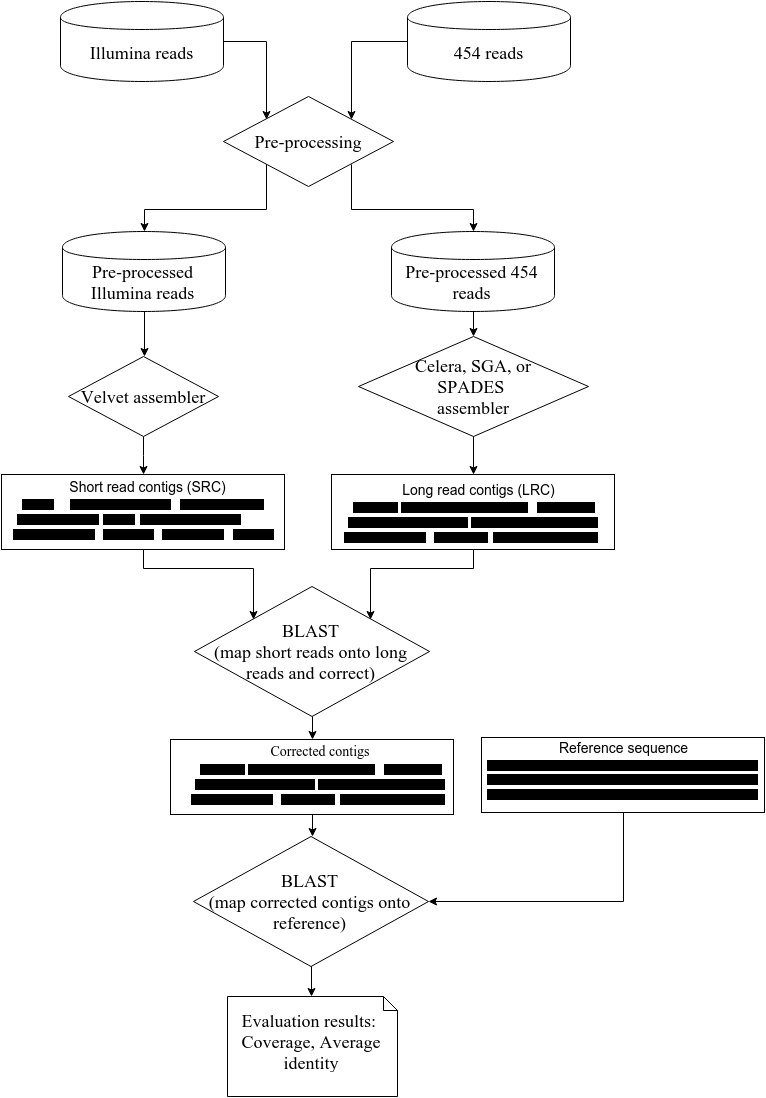
\includegraphics[width=12cm, height=18cm]{flowChart.png}}
\caption{Flow chart of the assembly improvement processes.}
\label{flowChart}
\end{figure*}


\begin{figure*}[htbp]
\centerline{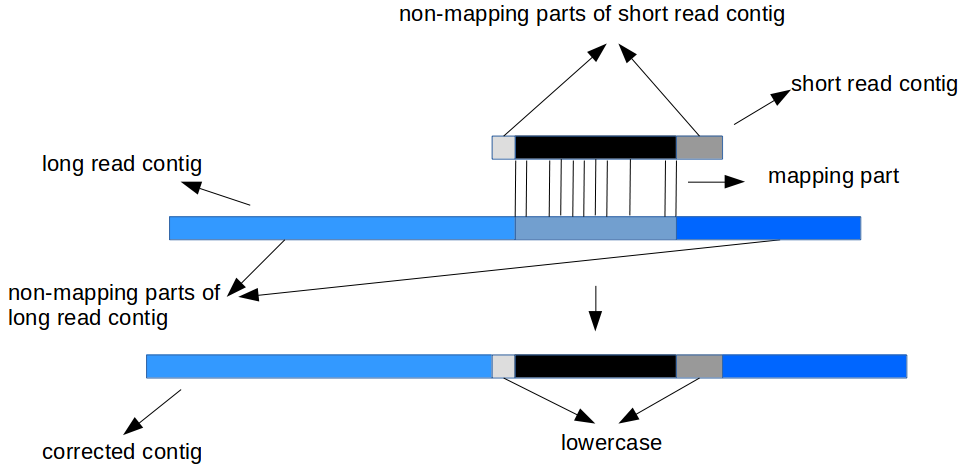
\includegraphics[width=12cm, height=5cm]{BACAlgorithm1.png}}
\caption{Correction method: Correct the long read contig according to the mapping information of the short read contig.}
\label{correction}
\end{figure*}

\ctable[star
	    center
      cap     = {},
      % 
      caption = {Results of assembly correction method on BAC data.},
      % 
      label   = {tab:resultsTable},
      doinside = \scriptsize,
      width = 1\textwidth,
      %maxwidth=19cm,
      %
      %
       pos = htb      
       ]
       {c>{\raggedright\arraybackslash}X>{\raggedright\arraybackslash}X>{\raggedright\arraybackslash}
         X>{\raggedright\arraybackslash}X>{\raggedright\arraybackslash}X>{\raggedright\arraybackslash}
         X>{\raggedright\arraybackslash}X>{\raggedright\arraybackslash}}
       {         
        \tnote[]{{\scriptsize Name: the name of the data group that constitute the assembly; \# of contigs: the number of contigs that belong to the resulting assembly; \# of Mapped Contigs: the number of contigs that successfully mapped onto the reference sequence; \# of Covered bases: the number of bases on the reference sequence that are covered by the assembly; Coverage: percentage of covered reference; Avg. identity: percentage of the correctly predicted reference bases; \# of Gaps: The number of gaps that cannot be covered on the reference genome; Size of Gaps: total number of bases on the gaps.}}
         \tnote[*]{{\scriptsize ``2'' represents the results of the second cycle of correction, ``3'' represents the third cycle.}}
       }
       {
         \FL
         Name & Length & \# of Contigs & \# of Mapped Contigs & \# of Covered bases & Coverage & Avg. Identity & \# of Gaps & Size of Gaps\ML
		 \textbf{\textit{Reference}} & \textit{176.843} & & & & & & & \ML
		 \addlinespace
		 \textbf{Velvet} & & & & & & & \NN
         Ill. Velvet & 197,040 & 455 & 437 & 175,172 & 0.99055 & 0.97523 & 39 & 1,671 \ML
         \textbf{Celera} & & & & & & & \NN       
         454 Celera & 908,008 & 735 & 735 & 172,563 & 0.97580 & 0.92599 & 18 & 4,280 \NN
         Ion Celera & 39,347 & 27 & 27 & 47,638 & 0.26938 & 0.96932 & 47 & 129,205 \ML
         \addlinespace
         \textbf{Corrected Celera} & & & & & & & \NN
         Ill-454 Celera & 371,065 & 250 & 250 & 176,071 & 0.995635 & 0.944558 & 5 & 772 \NN
         Ill-454 Celera^2\tmark[*] & 365,802 & 245 & 245 & 176,343 & 0.9971 & 0.9455 & 4 & 500 \NN
         Ill-Ion Celera & 93,909 & 30 & 28 & 81,819 & 0.46267 & 0.96327 & 36 & 95,024 \NN
         Ill-Ion Celera^2 & 145,262 & 30 & 28 & 91,962 & 0.52002 & 0.97412 & 33 & 84,881 \NN
         Ill-Ion Celera^3 & 216,167 & 30 & 28 & 99,645 & 0.56347 & 0.98066 & 34 & 77,198 \ML
         \textbf{SGA} & & & & & & & \NN
         454 SGA & 62,909,254 & 108,095 & 101,514 & 176,546 & 0.99832 & 0.97439 & 1 & 297 \NN
         Ion SGA & 842,997 & 6,417 & 6,122 & 153,092 & 0.86569 & 0.99124 & 197 & 23.751 \ML	
         \addlinespace
         \textbf{Corrected SGA} & & & & & & & \NN
         Ill-454 SGA & 295,009 & 335 & 335 & 176,757 & 0.99951 & 0.96823 & 5 & 86 \NN
%         Ill-454 SGA^2 & 279,034 & 305 & 305 & 176,757 & 0.99951 & 0.96769 & 5 & 86 \NN
         Ill-Ion SGA & 197,509 & 291 & 291 & 175,052 & 0.98987 & 0.97501 & 45 & 1,791 \NN
         Ill-Ion SGA^2 & 203,064 & 291 & 291 & 175,676 & 0.99340 & 0.97413 & 34 & 1,167 \ML
%         Ill-Ion SGA^3 & 204,524 & 291 & 291 & 175,677 & 0.99341 & 0.97405 & 34 & 1,166 \ML
         \textbf{SPADES} & & & & & & & \NN
         454 SPADES & 12,307,761 & 49,824 & 49,691 & 176,843 & 1.0 & 0.98053 & 0 & 0 \NN
         Ion SPADES & 176,561 & 110 & 107 & 167,890 & 0.94937 & 0.92909 & 9 & 8,953 \ML	
         \addlinespace
         \textbf{Corrected SPADES} & & & & & & & \NN
         Ill-454 SPADES & 290,702 & 298 & 298 & 176,454 & 0.99780 & 0.96538 & 5 & 389 \NN
%         Ill-454 SPADES^2 & 290,917 & 297 & 297 & 176,454 & 0.99780 & 0.96530 & 5 & 389 \NN
%         Ill-454 SPADES^3 & 291.653 & 297 & 297 & 176.454 & 0.99780 & 0.96527 & 5 & 389 \NN
         Ill-Ion SPADES & 198,665 & 52 & 52 & 171,977 & 0.97248 & 0.94215 & 4 & 4,866 \NN
         Ill-Ion SPADES^2 & 200,307 & 52 & 52 & 172,101 & 0.97319 & 0.94230 & 2 & 4,742 \ML
         \textbf{Masurca} & & & & & & & \NN
         Ill-454 Masurca & 380 & 1 & 0 & 0 & 0 & 0 & 0 & 0 \NN
         Ill-Ion Masurca & 2,640 & 8 & 8 & 1,952 & 0.01104 & 0.98223 & 9 & 174,891 \ML
 		\textbf{Celera-CABOG} & & & & & & & \NN
         Ill-454 Celera & 1,101,716 & 891 & 891 & 174,330 & 0.98579 & 0.92452 & 12 & 2,513 \NN
         Ill-Ion Celera & 0 & 0 & 0 & 0 & 0.0 & 0.0 & 0 & 0.0 \NN
         \LL
       }
\vspace*{-0.3cm}

\section{Results and Conclusion}
We presented the results on Table \ref{tab:resultsTable}. We interpreted the results in different categories. 

\subsection{454 vs. Ion-Torrent}
\label{454Ion}
As we see in Table \ref{tab:dataprop}, Ion-Torrent reads are shorter than 454 reads and they have less mean base quality. So, we did not expect to have better assembly with Ion-Torrent reads than 454 reads. The results in Table \ref{tab:resultsTable} agree with our expectations.
In Table \ref{tab:resultsTable}, we see that the assembly of 454 reads perform better on evaluation metrics than Ion-Torrent with all kind of assemblers. The assembly of Ion-Torrent reads with Celera assembler has very low coverage value: 26.94\%. The reason for the low coverage might be because Celera assembler is not designed for Ion-Torrent read type (shorter reads with lower quality), even 454 and Ion-Torrent reads have similar error types at the homopolymer regions. SGA assembly with Ion-Torrent reads perform better on Coverage (86.57\%) but it cannot reach to the Coverage of SGA assembly with 454 reads (99.83\%). The assembly of Ion-Torrent reads has the highest coverage with SPAdes assembler (94.94\%). Correction of the Ion-Torrent contigs improves the assembly quality but even after correction phase Ion-Torrent corrected assembly cannot reach the results of 454 corrected assembly. 

\subsection{Assemblers}

On Table \ref{tab:resultsTable}, the assembly obtained by Velvet with only short Illumina reads has good coverage rate (99\%) and average identity rate (97.5\%). The number of contigs with Velvet assembly is 455, of which 437 maps to the reference genome. There are 39 gaps and the total size of the gaps is 1,671. Our aim was to increase the coverage, improve the average identity and decrease the number of contigs and gaps, and shrink the lengths of the gaps.

Since we decided that 454 reads resulted better assembly than Ion-Torrent reads in Section \ref{454Ion}, we compared different assemblers through 454 contigs. The assembly of Celera with the 454 long reads has 97.5\% coverage and 92.6\% average identity, which are lower than Illumina-Velvet values. Contig number (735) is reasonable but gap number and size is quiet high (18; 4,280). 
SGA assembly with 454 reads has very high coverage (99.83\%) and identity (97.4\%). It has just one gap with size 297, but the number of contigs is also very high (101,514) which is an unwelcome situation. SPAdes-454 assembly has also high number of contigs (49,824) which completely cover the reference sequence with 98\% average identity. SPAdes has less contig numbers and higher coverage and average identity than SGA. 
If we evaluate the results according to the contig numbers, Celera-454 results seem more reasonable than SGA or SPAdes results, since it has reasonable number of contigs even with low coverage and average identity.

\subsection{Correction Method}

It is obvious that the correction method improved the 454 and also Ion-Torrent read assemblies with all kind of assemblers (Table \ref{tab:resultsTable}). Now we will just mention on 454 read assemblies for simplicity.

When we applied our correction method on Celera-454 assembly with the Velvet-Illumina assembly, we achieved better coverage and average identity rates: the coverage of 454 assembly increases up to 99.7\% and the average identity rate increases up to 94.4\% on the first correction cycle. The second correction cycle increases the coverage and average identity rates up to 99.7\% and 94.5\% and convergences. The number of contigs decrease down to 245 from 735, and the gap number decreases down to 4 with total size 500 from 18 (size:4,280). Since the third correction cycle does not give better results it is not given on Table \ref{tab:resultsTable}.

Our correction method increases the coverage of SGA-454 assembly up to 99.9\% from 99.8\% but with less average identity and with more gaps even the total size of the gaps is shorter. Correction with the short read assembly decreases the contig number down to a reasonable number (335). Corrected SGA assembly has the largest coverage rate among all, and it is also better than Velvet-Illumina assembly.

The number of contigs in SPAdes assembly is also decreased to 298 from 49,691 with the correction method. With the decrease in contig numbers the coverage also decreased (99.7\%) as well as average identity (96.5\%). The gap number increased to 5 from 0 with total size 389.

So, in all kind of assemblers' results we saw that assembly correction by using advantages of different technologies improves the resulting assembly.

\subsection{Hybrid Assemblers}

We also wondered the results of two hybrid assemblers on our multiple type of data. We ran Masurca and Celera-CABOG with default parameters given two groups of hybrid data as input: Illumina \& 454 and Illumina \& Ion-Torrent. Hybrid assemblers Masurca and CABOG did not have good assembly rates. We got zero coverage rate with 454 and Illumina reads with Masurca. The only contig left after the contamination removal did not map to the reference sequence. We also got very low coverage (1.1\%) with 98.2\% average identity  with Ion-Torrent \& Illumina reads. So, we can say Masurca did not work very well in our case with our data types. 

We got 0\% coverage with Ion-Torrent \& Illumina with CABOG. All of the resulting contigs obtained from the assembly were removed as contamination. CABOG did not work well on Illumina \& Ion-Torrent but it worked pretty good on Illumina \& 454 with 98.58\% coverage and 92.5\% average identity. It has 891 contigs and 12 gaps with total size 2,513. Still, it can not catch the corrected assembly results.

\section{Conclusion}

We presented a new method to improve draft assemblies by correcting high contiguity assemblies using the contigs obtained with high quality reads. Assembling short and long reads seperately with de Bruijn graph based and OLC graph based assemblers according to data types and then using correction methods like this one on the resulting assemblies give better results than just using hybrid assemblers with both short and long reads. Our method is useful and it gives better results than using all data for once with a hybrid assembler. 

However, the need to develop new methods that exploit different data properties of different HTS technologies, such as short/long reads or high/low quality of reads, remains. In this manner, as future work, our correction algorithm can be improved by exploiting the paired end information of the short, high quality reads after the correction phase, to fill in the gaps between corrected contigs.

\paragraph{Funding.}

The project is supported by the Republic of Turkey Ministry of Development Infrastructure Grant (no: 2011K120020), BİLGEM TÜBİTAK (The Scientific and Technological Research Council of Turkey) grant (no: T439000), and a TÜBİTAK grant to C.A.(112E135).\\

%\newpage
%
% ---- Bibliography ----
%
\begin{thebibliography}{}
%

\bibitem{ssake:2007} R.L.Warren, G.G.Sutton, S.J.M.Jones, R.A.Holt: Assembling millions of short DNA sequences using SSAKE, Bioinformatics, 23(4):500-501 (2007)
\bibitem{sharcgs:2007} J.C.Dohm, C.Lottaz, T.Borodina, H.Himmelbauer: SHARCGS, a fast and highly accurate short-read assembly algorithm for de novo genomic sequencing, Genome Research, 17(11):1697-1706 (2007)
\bibitem{vcake:2007} W.R.Jeck, J.A.Reinhardt, D.A.Baltrus, M.T.Hickenbotham, V.Magrini, E.R.Mardis, J.L.Dangl, C.D.Jones: Extending assembly of short DNA sequences to handle error, Bioinformatics, 23(21):2942-2944 (2007)
\bibitem{hapsemblerDonmez:2011} N.Donmez, M.Brudno: Hapsembler: An Assembler for Highly Polymorphic Genomes, Proceedings of the 15th Annual International Conference on Research in Computational Molecular Biology, pages:38-52 (2008)
\bibitem{celera:2000} E.W.Myers, G.G.Sutton, A.L.Delcher, I.M.Dew, D.P.Fasulo, M.J.Flanigan, S.A.Kravitz, C.M.Mobarry \textit{et~al}: A Whole-Genome Assembly of Drosophila, Science, {287(no:5461)}:2196-2204, doi:10.1126/science.287.5461.2196 (2000)
\bibitem{sga:2012} J.Simpson R.Durbin: Efficient \textit{de novo} Assembly of Large Genomes Using Compressed Data Structures, Genome Research, {22}:549-556, doi:10.1101/gr.126953.111 (2012)
\bibitem{velvetZerbino:2008} D.R.Zerbino, E.Birney: Velvet: Algorithms for \textit{de novo} Short Read Assembly Using de Bruijn Graphs, Genome Research, {18(5)}:821-829, doi: 10.1101/gr.074492.107 (2000)
\bibitem{spadesBankevich:2012} A.Bankevich, S.Nurk, D.Antipov, A.A. Gurevich, M.Dvorkin, A.S.Kulikov, V.M.Lesin, S.I.Nikolenko {\it et~al}: SPAdes: A New Genome Assembly Algorithm and Its Applications to Single-Cell Sequencing, Journal of Computational Biology, {19(5)}:455-477, doi:10.1089/cmb.2012.0021 (2012)
\bibitem{allpaths:2008} J.Butler, I.MacCallum, M.Kleber, I.A.Shlyakhter, M.K.Belmonte, E.S.Lander, C.Nusbaum, D.B.Jaffe: ALLPATHS: \textit{De novo} Assembly of Whole-Genome Shotgun Microreads, Genome Research, {18(5)}:810-820, doi:10.1101/gr.7337908 (2008)
\bibitem{abyssSimpson:2009} J.T.Simpson, K.Wong, S.D.Jackman, J.E.Schein, S.J.M.Jones, İ.Birol ABySS: A parallel assembler for short read sequence data, Genome Research, 19(6):1117-1123 (2009)
\bibitem{eulerPevzner:2008} M.J.Chaisson, D.Brinza, P.A.Pevzner: De novo fragment assembly with short mate-paired reads: Does the read length matter?, Genome Research, 19(2):336-346 (2008)
\bibitem{cabogMiller:2008} J.R.Miller, A.L.Delcher, S.Koren, E.Venter, B.P.Walenz, A.Brownley, J.Johnson, K.Li, C.Mobarry, G.Sutton: Aggressive Assembly of Pyrosequencing Reads with Mates, Bioinformatics, {24(24)}:2818-2824, doi:10.1093/bioinformatics/btn548 (2008)
\bibitem{masurcaZimin:2013} A.Zimin, G.Mar\c{c}ais, D.Puiu, M.Roberts, S.L.Salzberg, J.A.Yorke: The MaSuRCA Genome Assembler, Bioinformatics, {29(21)}:2669-2677, doi:10.1093/bioinformatics/btt476 (2013)
\bibitem{mira} B.Chevreux, T.Wetter, S.Suhai:  Genome Sequence Assembly Using Trace Signals and Additional Sequence Information, Computer Science and Biology:Proceedings of the German Conference on Bioinformatics (GCB), {99}:45-56 (1999)
\bibitem{miraest} B.Chevreux, T.Pfisterer, B.Drescher, AJ.Driesel, WE.Müller, T.Wetter, S.Suhai: Using the miraEST assembler for reliable and automated mRNA transcript assembly and SNP detection in sequenced ESTs, Genome Research, 14(6), 1147-1159 (2004)
\bibitem{cerulian:2013} V.Deshpande, E.D.Fung, S.Pham, V.Bafna: Cerulean: A hybrid assembly using high throughput short and long reads, arXiv:1307.7933 [q-bio.QM] (2013)
\bibitem{BACRef} B.Ergüner, D.Ustek, MŞ. Sağıroğlu: Performance Comparison of Next Generation Sequencing Platforms, Poster presented at: 37th International Conference of the IEEE Engineering in Medicine and Biology Society (2015)
\bibitem{wang:2012} Y.Wang, Y.Yao, P.Bohu, H.Pei, L.Yixue, S.Zhifeng, X.Xiaogang, L.Xuan: Optimizing Hybrid Assembly of Next-Generation Sequence Data from Enterococcus Faecium: a Microbe with Highly Divergent Genome, BMC Systems Biology, {6(Suppl 3)}:S21, doi:10.1186/1752-0509-6-S3-S21 (2012)
\bibitem{blast} S.Altschul, W.Gish, W.Miller, E.Myers, D.J.Lipman: Basic Local Alignment Search Tool, Journal of Molecular Biology, {215(3)}:403-410 (1990)




\end{thebibliography}
\clearpage
\addtocmark[2]{Author Index} % additional numbered TOC entry
\renewcommand{\indexname}{Author Index}
\printindex
\clearpage
\addtocmark[2]{Subject Index} % additional numbered TOC entry
\markboth{Subject Index}{Subject Index}
\renewcommand{\indexname}{Subject Index}
%\input{subjidx.ind}
\end{document}
